\section{Design}\label{sec: Design}
In this section the design and decisions that where made to achieve the laboratory are discussed.
%The code for lab 03 can be reviewed online under the flowing link \href{https://github.com/haringd/EGR680_FPGA_Labs/tree/master/VENDMACH}{http://github.com/haringd/EGR680\_FPGA\_Labs/tree/master/VENDMACH}.
\subsection{SDK Lab specification}\label{subsec: Vending machine specification}
In this part, you will create a simple hardcore ARM Cortex-A9 based embedded system on the PYNQ board. The
embedded system design is broken up into three parts: Hardware design of the ARM Cortex-A9 hardcore
processor, application software design using SDK, and finally hardware implementation of the software running
on the hardcore processor. The application you will design in this part is a UART application that prints “HELLO
WORLD” to a terminal emulator like Tera Term. Use the figure below as a flow guide for this lab. The diagram
for the completed design is shown in Figure \ref{fig: Vivado_lab4_CompletedDesign}. 
\begin{figure}[H]
	\centering
	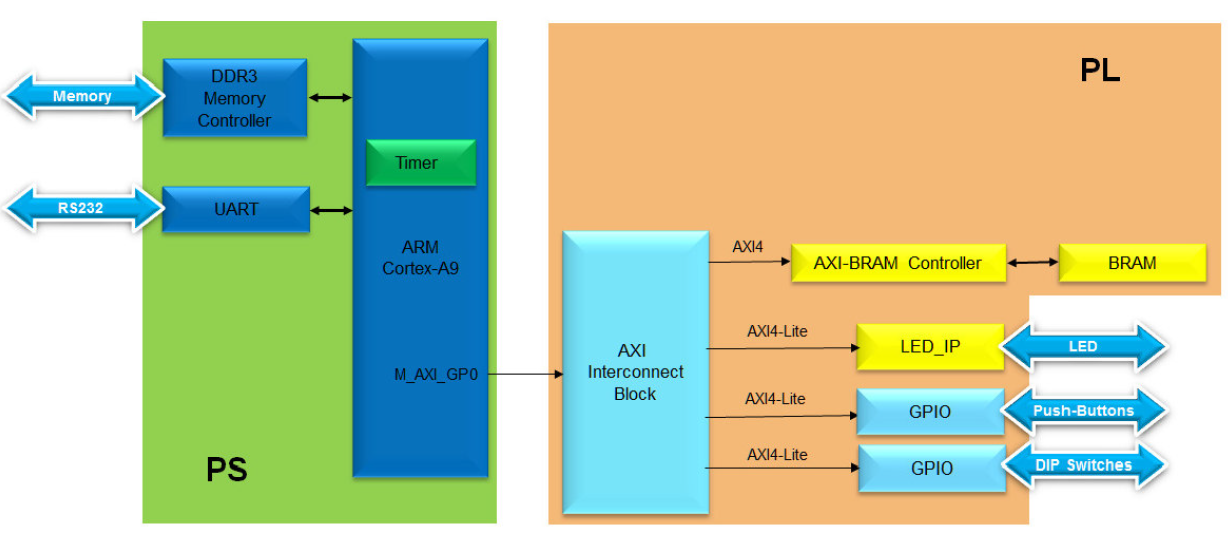
\includegraphics[width=1.0\textwidth]{01_images/Vivado_lab4_CompletedDesign.PNG}
	\caption{Completed Design.}
	\label{fig: Vivado_lab4_CompletedDesign}
\end{figure}

\subsection{HDL}\label{subsec: HDL}
Figure \ref{fig: Vivado_lab_HDL_topView} shows the HDL top level based of the ZYNQ 7 Processing system which is connected with an AXI bus S00\_AXI to a intellectual property (IP) block that manages peripherals. From there an AXI bus is used to connect two general purpose input output (GPIO) IP blocks, one for buttons and another one for switches. Furthermore, a Processor System Reset IP block is used that interconnects all resets.
\begin{figure}[H]
	\centering
	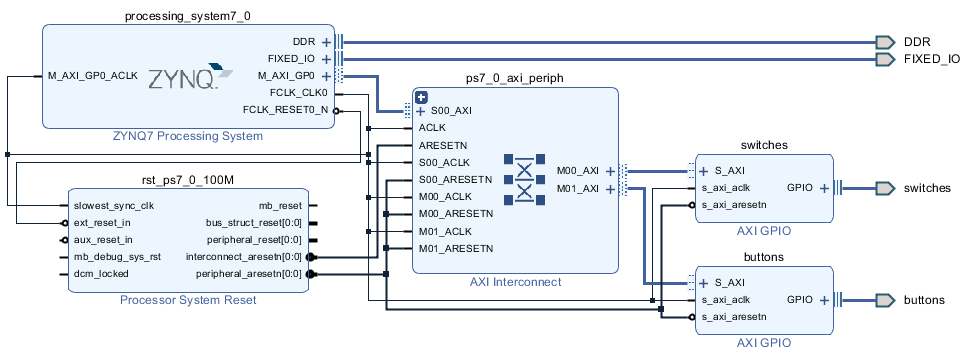
\includegraphics[width=1.0\textwidth]{01_images/Vivado_lab_HDL_topView.PNG}
	\caption{HDL Top Level Design.}
	\label{fig: Vivado_lab_HDL_topView}
\end{figure}

\subsection{SDK}\label{subsec: SDK}
After the HDL top level is defined the SDK can be launched with \textbf{File $\rightarrow$ Launch SDK}. The *.hdf file should be shown or can be opened that shows the base registers for the switches and buttons, as highlighted in Figure \ref{fig: Vivado_lab4_SW_BTN_Register}. 
\begin{figure}[H]
	\centering
	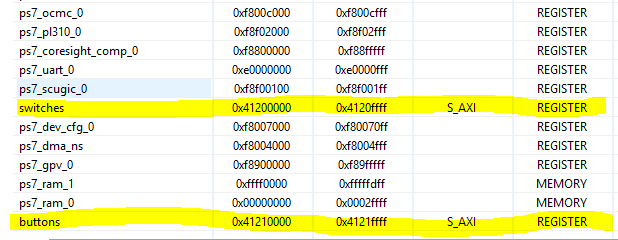
\includegraphics[width=1.0\textwidth]{01_images/Vivado_lab4_SW_BTN_Register.PNG}
	\caption{*.hdf file that shows the base register for switches and buttons.}
	\label{fig: Vivado_lab4_SW_BTN_Register}
\end{figure}

After writing the C code given in part two and loading the the bit stream file and the build elf file onto the board the serial console Terra Term shows the status of the buttons and switches, as shown in Figure \ref{fig: Vivado_lab4_TT_PartII}
\begin{figure}[H]
	\centering
	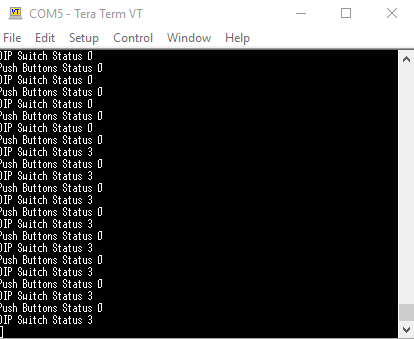
\includegraphics[width=0.7\textwidth]{01_images/Vivado_lab4_TT_PartII.PNG}
	\caption{Terra Term print out of the switches and buttons status.}
	\label{fig: Vivado_lab4_TT_PartII}
\end{figure}

\subsection{Let's Make a Deal}\label{subsec: Lets Make a Deal}
Part III of laboratory 4 is to program a game show named "Let's Make a Deal!". 
Therefor, the previous HDL code is reused because the push buttons (psb) and universal asynchronous receiver transmitter (UART) is used for the game show while the switches are just not initials in the program code and not used. 

The game works as followed a computer, in this case ZYNQ embedded system, uses based on the users input time. The $startTime$ stamp is made as the game starts while the $stopTime$ stamp is made as the user presses the input button, the $deltaTime$ is calculated according Equation \ref{eq: delta}. A random number is generated out of the $deltaTime$ stamp that is determined according to Equation \ref{eq: random}. The user input is to chose a door which hides a good deal but to get it the users answer has to match the computers generated door number.

The program consist of two switch case statements one for the program flow as shown in Figure \ref{fig: Game Show state machine}. The second state machine contains the input logic to map the binary button input to a integer number. In addition, simple delays where used to de-bounce the buttons.  

The four buttons are configured as the following btn0 is Door 1, btn1 is Door 2, btn2 is Door 3, btn3 is Door 4.

The complete code listening can be found under Section \ref{subsec: C code}.
\\
\\
\textbf{IMPORTANT:} For the game show the programmable logic has to be flashed first with the generated bit stream file than the compiled C code can be flashed with the *.elf file.

\begin{equation}
deltaTime = startTime - stopTime \label{eq: delta}
\end{equation}
\begin{equation}
rnd = (deltaTime\ \%\ 4) + 1 \label{eq: random}
\end{equation}

\subsection{Game Show State Machine}\label{subsec: Game Show State Machin}
\begin{figure}[H]
	\begin{verbatim}       
/*********************************************************************************
** FSM State machine                                                            **
**********************************************************************************
                   000                        
+---------------------+           
| Idle                |           
| Display user input  |<--------+
|                     |         | 
+---------------------+         | 
    |                           |             
    |                           |             
    |              001          |             
+---------------------+         |        
|                     |         |        
| Wait for button     |         |        
| coin_val on Pmod A  |         |        
+---------------------+         |                           
    |                           |             
    |                           |             
    |              002          |             
+---------------------+         |             
| user output         |         |             
| if (rnd == door)    |---------+
| Display output      |                       
+---------------------+                            
/*********************************************************************************/
	\end{verbatim}
	\caption{Game Show state machine.}\label{fig: Game Show state machine}
\end{figure}

